\SSbreak\\
\emph{Source: Italian Team Competition Final 2020}\\
\emph{Proposer: \Pmatt}\\ 
\emph{Problem ID: 124}\\
\emph{Date: 2021-02-06}\\
\emph{Difficulty: Challenging}\\
\SSbreak

\SSpsetQ{
For a triangle \(ABC\), let \(P\) be on \(AB\), and \(X\) be the circumcenter of \(APC\), \(Y\) be the circumcenter of \(BPC\), and \(Z\) be the intersection of \(AX\) and \(BY\). Given that \(AB=91\), \(BC=104\), and \(CA=65\), what is the length of \(CZ\)?
}\bigskip

\begin{solution}\hfil\medskip

    \begin{figure}[h!]
        \centering
    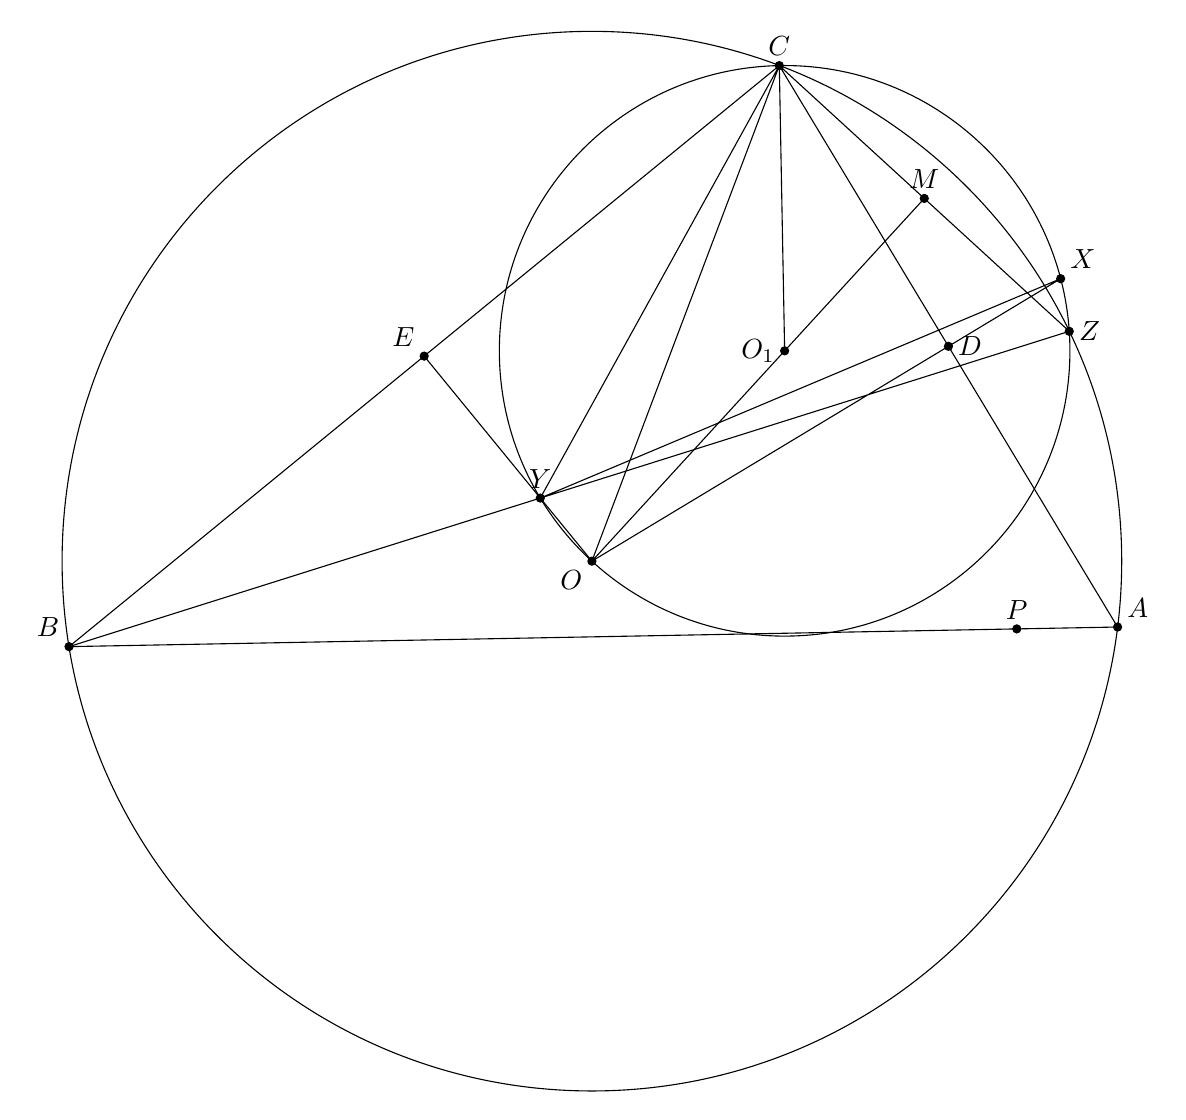
\begin{tikzpicture}[scale = 0.0045cm]
    \def\A{(-73.1687,-160.74487)}
    \def\B{(-177.150601,-162.690109)} 
    \def\C{(-106.716,-105.07095)}
    \def\P{(-83.167045,-160.931914)} 
    \def\Y{(-130.41799645,-147.9570)} 
    \def\Z{(-77.96303196,-131.419898)} 
    \def\O{(-125.3000,-154.21325)}
    \def\X{(-78.81585,-126.20343707)}
    \def\o{(-106.186855,-133.356169)} 
    \def\M{(-92.33951608,-118.2454)} 
    \def\D{(-89.94239,-132.9079)}
    \def\E{(-141.9333,-133.880532)}
    \filldraw \B circle (0.4) node[above left] {$B$}; %B
    \filldraw \A circle (0.4) node[above right] {$A$}; %A
    \filldraw \C circle (0.4) node[above] {$C$}; %C
    \filldraw \X circle (0.4) node[above right] {$X$}; %X
    \filldraw \P circle (0.4) node[above] {$P$}; %P
    \filldraw \Y circle (0.4) node[above] {$Y$}; %Y
    \filldraw \Z circle (0.4) node[right] {$Z$}; %Z
    \filldraw \O circle (0.4) node[below left] {$O$}; %O
    \filldraw \o circle (0.4) node[left] {$O_1$}; %o
    \filldraw \M circle (0.4) node[above] {$M$}; %M
    \filldraw \D circle (0.4) node[right] {$D$}; %D
    \filldraw \E circle (0.4) node[above left] {$E$}; %E
    \draw (-125.3000,-154.21325) circle (52.53887);
    \draw (-106.186855,-133.356169) circle (28.29016);
    \draw \E -- \B -- \A -- \C -- \E -- \Y -- \C  -- \Z -- \Y -- \X -- \O -- \C -- \o;
    \draw \B -- \Y -- \O -- \M;
    \end{tikzpicture}
    \end{figure}


    By simple angle chasing $\triangle CXA$ and $\triangle CYB$ are similar, we have $\angle ZAC=\angle XAC=\angle YBC=\angle ZBC$, so $Z$ is on $\odot (ABC)$. Standard calculations on $\triangle ACX$ and $\triangle ABC$ give $\text{sin}(\angle ZAC)=\frac{3\sqrt{3}}{14}$ and $R_{\odot (ABC)}=\frac{91\sqrt{3}}{3}$, so $CZ= 2R_{\odot (ABC)}\text{sin}(\angle ZAC)=39$
\end{solution}\bigskip
